\documentclass[review]{elsarticle} % doble espacio
%\documentclass{elsarticle}

\biboptions{sort&compress}

\usepackage{dingbat}
\usepackage{graphicx,url,hyperref,doi}

\begin{document}

\author{Alexander {Espronceda Gómez}, Satu {Elisa Schaeffer}}

\date{\today}


\let\today\relax
\makeatletter
\def\ps@pprintTitle{%
    \let\@oddhead\@empty
    \let\@evenhead\@empty
    \def\@oddfoot{\footnotesize\itshape
         {} \hfill\today}%
    \let\@evenfoot\@oddfoot
    }
\makeatother

\bibliographystyle{mighelnat}

\title{Sentiment Analysis through Conversational Data}
\address{San Nicolás de los Garza, Nuevo León, México}

\begin{abstract}
In this thesis, open-sourced software is proposed, which interprets the text entered by a person and determines how they are feeling at the moment, with the purpose of being used in tandem with another software or algorithms focused on conversational data.

The study method used will make a comprehensive analysis of neural networks, as well as pattern recognition and data collection.
The algorithm is open-source so anyone can add or remove modules as needed.

\vspace*{0.5cm}
\textit{Key Words: } Sentiment Analysis, Machine Learning, LSTM Neural Network, Conversational Data, Open-Source Code


\end{abstract}

\maketitle

\section{Introduction}

Human beings are social beings, this is widely known. To survive, we must band together and communicate with each other, bonding in the process. This is thanks to a neural process called \textit{empathy}, which is defined as a three-part process that happens in our brains \citep{rf1}. That happens roughly like this:
\begin{itemize}
	\item Emotional simulation centered in the limbic system, which makes us mirror the emotional elements we're watching.
	\item Processing the perspective in the prefrontal and temporal cortex.
	\item Assessing the course of action to take, either showing compassion or doing something else. This is assumed to be based in the obitofrontal cortex, as well as several other parts of the brain.	
\end{itemize}
\begin{figure}[!h]
	\centering
	\includegraphics[scale=0.2]{BrainMap}
	\caption[Lateral brain map of the parts in charge of empathy processes.]{Lateral brain map of the parts in charge of the empathy processes. Gray and pink are parts of the limbic system, cyan is part of the prefrontal cortex, green is part of the temporal cortex, blue is part of the orbitofrontal cortex. Drawing generated using BrainPainter \citep{img1}.}
	\label{fig:brainmap}
\end{figure}
This is clearly what is usually considered a human-only behavior, but there are studies that indicate that apes, dogs and rodents have been observed to take action at the presence of distress signals, either from humans or other members of their own species \citep{rf2}.
If this is true, theoretically, a machine could be taught to process signals of distress and react accordingly using a learning algorithm.
\pagebreak

\section{Hypothesis}
The hypothesis of this thesis is that using supervised machine learning with a neural network could accurately classify the sentiment behind an input text as ``Good'', ``Neutral'' or ``Bad'', with the purpose of being implemented in tandem with another software or algorithms focused on conversational data.

\section{Background}
In this section some of the key concepts of this project are described for better comprehension of it as a whole.
\subsection{Basic Concepts}
\begin{description}
	\item[Machine Learning]{Also known as ML. The type of algorithm needed for automatic processing, making the machine ``learn'' (hence the name) over time given enough data.}
	\item[Neural Network]{A Machine Learning algorithm that uses weights and filters to output data.}
	\item[Natural Language Processing]{This is the method used for the algorithm to understand the content of the sentences, this is usually achieved by using tokenization but a preset corpus can also be used.}	
	\item[Sentiment Analysis]{This involves a ML algorithm, usually a Neural Network, that is able to analyze sentences and classify them according to the words used.}
	\item[Corpus]{Preset internal dictionary that the algorithm uses.}
	\item[Tokenizing]{Process that converts every word in the lexicon to an assigned number for easier processing}
\end{description}

\subsection{Supervised Machine Learning}
Supervised ML can be described, broadly and figuratively speaking, as a black box where some data is inserted as an input and numbers come out of it as an output \citep{rf8}. This output, as opposed to other types of Machine Learning, is later analyzed and compared to real life data. This means this type of ML is best used as an auxiliary tool more than the main source of information from a process.
Some more advanced models of ML allow some internal parameters inside this figurative black box to be able to be tampered with, so that some characteristics of the input data can have effect on the output, these parameters are called \textit{weights} \citep{rf9}.
Most ML algorithms have two stages: training and validation:
\begin{itemize}
\item Training processes the inputs and makes educated guesses, and in case of guessing incorrectly, depending on the obtained result, the weights are changed accordingly.
\item Validation is as simple as it sounds, some input is fed to the algorithm and information needs to be compared to the real results to test the accuracy percentage.
\end{itemize}
One of these models that is one of the most used nowadays is the one called \textit{Neural Network}.

\subsection{Neural Network}
A neural network works by using \textit{neurons} that utilize layers that individually weigh the input given to them from the initial text or, if this has been processed already, from another neuron \citep{rf9}.
Likewise, similar to how biological brains work, these algorithms can only predict reliably if given enough data to train and validate their outputs with.

\subsection{Sentiment Analysis}
Sentiment Analysis (or Opinion Mining, as it is also known) as a tool for data analysis is arguably a recent happening. The term was coined in 2003 and has evolved ever since \citep{rf3}.
This type of data analysis has a lot of potential usages that have yet to be implemented in the daily life.

The specific execution of the algorithm varies depending on the intended purpose, but the concept and process that is used is generally the same:
\begin{itemize}
	\item The sentence to analyze is broken down to its component parts, this process is called \textit{tokenization}, and the resulting products are called, fittingly, \textit{tokens}.
	\item Every token is then tagged, making it part of an internal dictionary or \textit{lexicon}
	\item A score is assigned to every token depending on the used dataset.
\end{itemize}
The end score could be left as-is or can be reintroduced to the algorithm for a multi-layered approach depending on its focus \citep{rf4}.

\subsection{Tokenizing}
Tokenizing is the process that happens while making tokens, the way it works is very straightforward: every word in the lexicon that a machine can read is assigned a number for easier reading. Taking the following example:
\begin{center}
\fbox{This is an example text}
\end{center}

We can tell there are 5 words in the example phrase. So the tokenizing process would make the example look in the following way:
\begin{center}
\fbox{1,	2,	3,	4,	5}
\end{center}

\noindent where 1 corresponds to the word ``This'', 2 corresponds to ``is'', 3 to ``an'' and so on.

The interesting part about this process would happen if we used another example phrase, like the following:
\begin{center}
\fbox{This is another example}
\end{center}

If we did the tokenization process, it would be processed in this way:
\begin{center}
\fbox{1,	2,	6,	4}
\end{center}

Since the internal lexicon already knows some of the words in this second example, it reuses their token, adding new ones (in this example, ``another'' is 6) if needed.\\

This is fairly useful for a machine learning algorithm, since it will not have to compare such massive amount of characters in a string each time, and it would only need to evaluate integers. Whether its focus is either frequency or comparison.

\section{Related work}
In this section, some literature is listed which proposes projects which have similar approaches to the present work, and some others that may not have the same objectives in mind but use algorithms that could be applied as well.
\subsection{Similar Approaches}
\citet{rf10} describe three different text classificators with a focus on sentiment analysis from Twitter:\\ 
\begin{itemize}
\item Twitter Sentiment, which uses a Maximum Entropy algorithm\footnote{This algorithm works by having the bias that certain characteristics repeat more in certain categories in text. If no bias is found, the distribution is uniform \citep{rf17}.}.
\item Tweet Sentiments, which uses Support Vector Machines\footnote{Binary algorithm that can sort between two classes, or opt for classification in a ``one-versus-everything else'' basis \citep{rf18}.} for classifications.
\item Lingpipe, which uses both previous algorithms and also Naive Bayes\footnote{This algorithm utilizes weights expressed in \textit{-1}, \textit{0}, or \textit{+1} depending on the sensitivity of specific characteristics \citep{rf19}. Works very similarly to a classic perceptron, which only uses\\ \textit{0} or \textit{1}.}
\end{itemize}
\citet{rf6} mention Koko, which uses the OpenAI API which is a counseling app for distressed teenagers in need of immediate psychological support, composed of a chatbot and sentiment analysis capabilities while
\citet{rf14} propose a chatbot developed to comprehend instructions, classifying them internally with a predefined bank of words, and reacting accordingly.

\subsection{Sentiment Analysis in Other Areas}
\citet{rf5} draft out a movie review algorithm that was capable of detecting if the review was either positive or negative depending on the words used, and,
\citet{rf12} propose an algorithm that correlated the air pollution levels with the sentiment expressed in people's tweets.
\citet{rf13} mention a hierarchical attention network to detect the polarity of a customer's review, with the added bonus of being capable of learning from new data.
\citet{rf15} propose an algorithm that can detect hate speech in text using natural language text classification across several topics.
\citet{rf11} write about a classification system to detect if a tweet was deemed as extremist or non-extremist depending on the vocabulary used and a deep-learning algorithm. Similarly, \citet{rf16} report a Recurrent Neural Network that detect political statements in YouTube comments while also classifying them in \textit{positive}, \textit{negative}, or \textit{other} depending on the topic.

\subsection{Opportunities for Improvement}
One of the main positives of working with TensorFlow is the fact that it is a highly reusable code that can very much be ported to any system that can run Python.\\
It is important to mention GPT-3 as a whole, the framework that Koko -- mentioned by \citet{rf6} -- uses is, to date, one of the most impressive AI algorithm to be developed, the downsides being that, being still in beta phase, is very resource-heavy, and its access is reserved to businesses through a fee, very expensive to use for the general public, especially students. That is why in this project, TensorFlow is used, which is free to use, does not need a lot of resources to work and has the advantages of being portable once trained, and also being easily modifiable if needed.
\begin{table}[!h]
	\caption[Comparison between existing literature and the present work.]{Comparison between existing literature and the present work: \checkmark indicates the fulfillment of a criterion, otherwise $\times$ is used.}
	\vspace{0.5cm}
	\centering
	\begin{tabular}[t]{|l|l|l|l|l|l|}
	\hline
		\textbf{Project} & \rotatebox{90}{\textbf{Neural Network}} & \rotatebox{90}{\textbf{Text Processing}} & \rotatebox{90}{\textbf{Sentiment Analysis }} & \rotatebox{90}{\textbf{Open Source}} & \rotatebox{90}{\textbf{Modular}}
	\\ \hline
	\citet{rf10} Maximum Entropy & \checkmark & \checkmark & \checkmark & $\times$ & $\times$
	\\ \hline
	\citet{rf10} Support Vector Machines & \checkmark & \checkmark & \checkmark & $\times$ & $\times$
	\\ \hline
	\citet{rf10} Lingpipe & \checkmark & \checkmark & \checkmark &  $\times$ & $\times$
	\\ \hline
	\citet{rf6} & \checkmark & \checkmark & \checkmark &  $\times$ & $\times$
	\\ \hline
	\citet{rf14} & \checkmark & \checkmark & $\times$ & \checkmark & $\times$
	\\ \hline
	\citet{rf5} & \checkmark & \checkmark & \checkmark & \checkmark & $\times$
	\\ \hline
	\citet{rf11} & \checkmark & \checkmark & $\times$ &  \checkmark & $\times$
	\\ \hline
	\citet{rf12} & \checkmark & \checkmark & \checkmark &  \checkmark & $\times$
	\\ \hline
	\citet{rf13} & \checkmark & \checkmark & \checkmark & $\times$ & $\times$
	\\ \hline
	\citet{rf15} & \checkmark & \checkmark & $\times$ &  \checkmark & $\times$
	\\ \hline
	\citet{rf16} & \checkmark & \checkmark & \checkmark & \checkmark & $\times$
	\\ \hline
	The present work & \checkmark & \checkmark & \checkmark & \checkmark & \checkmark
	\\ \hline
	\end{tabular}
\end{table}
\pagebreak

\section{Proposed solution}
This project is built on Python v3.8.10, The libraries used for this project to come to fruition are TensorFlow v2.6.0 and Keras v2.6.0 for the Neural Network section and Natural Language Toolkit v3.5 (also known as NLTK) for the tokenization and stemming process.
\begin{figure}[!h]
	\centering
	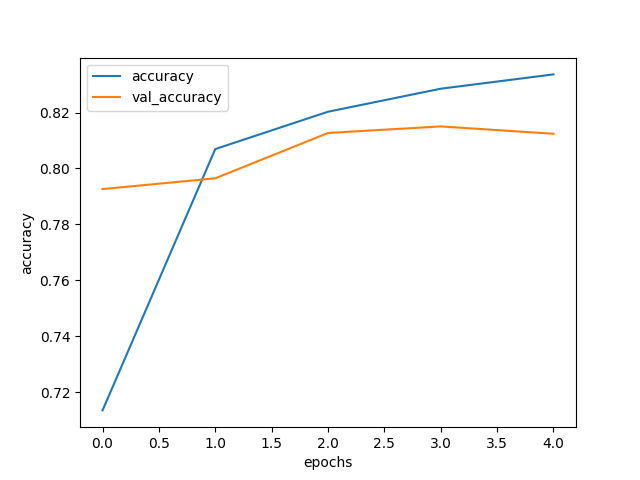
\includegraphics[scale=0.6]{Accuracy_Exp9}
	\label{fig:AccExp9}
	\caption{Accuracy values of the finished project}
\end{figure}
\begin{figure}[!h]
	\centering
	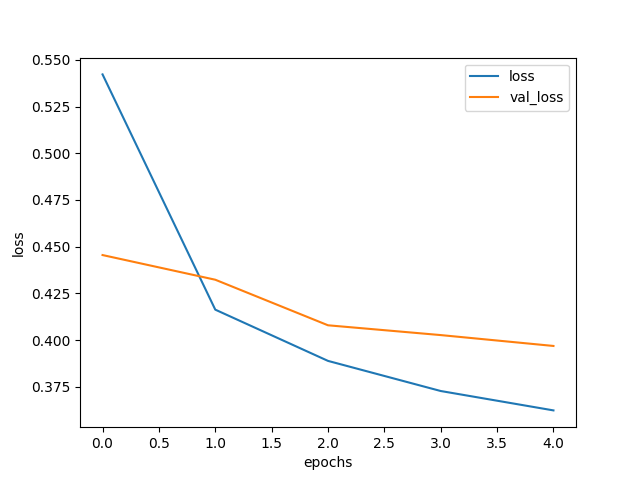
\includegraphics[scale=0.6]{Loss_Exp9}
	\label{fig:LossExp9}
	\caption{Loss values of the finished project}
\end{figure}
\pagebreak

\section{Evaluation}
In this section, various experiments of this project are shown with varying training data and parameters with the respective accuracy and loss values.
The purpose of these experiments is to determine if the parameters chosen for this project are optimal and, if not, correct them and know the reason behind the improvement.
The parameters that could potentially have a great impact on the output of the classification -- and therefore are the best to experiment with -- are the following:
\begin{itemize}
	\item Used datasets: This could influentiate the amount of words in the corpus and have a big impact on how some words are percieved
	\item Training epochs: How many loops does the algorithm go through before being considered fully trained, if this number is too high it could result in \textit{overfitting}, which is, in casual terms, the Neural Network equivalent of overthinking.
	\item Units in the LSTM layer: This unit system, albeit small in the overall scale of things, could make-or-break the algorithm if not tuned correctly.
	\item Categorized sentiments: Reducing the scope of the project could potentially benefit the overall accuracy of the remaining sentiments.
\end{itemize}

Lower loss and higher accuracy are preferred.
\subsection{Experiment Results}
\begin{itemize}
\item Experiment 1: Base Experiment: Base version of this thesis' project.
\item Experiment 2: More Datasets With Reduced Data Scope: This experiment takes sentences from one more dataset and 3 less categorized sentiments: ``Fear'', ``Joy'', and ``Love''.
\item Experiment 3: Augmented LSTM Units: Largely the same as Experiment 2, but the LSTM has more units to work with.
\item Experiment 4: Augmented Datasets Without Reduced Data Scope: A mix between Experiment 1 and 2. Three datasets with the full sentiment categorization and LSTM with 32 units.
\item Experiment 5: Reduced Classification Scope: This is the largest change on an experiment, the ``Neutral'' category has been completely disabled with the purpose of seeing how the rest of the data would be classified as.
\item Experiment 6: Reduced Epochs: Largely the same as previous experiments with half the epochs. This with the purpose of seeing if the data had been overfit.
\item Experiment 7: Added Stop Words: Same as Experiment 6, the difference being that the top 3 most recurrent words in the datasets are flagged as stop words in an attempt to mitigate the bleed between categories.
\item Experiment 8: Extra Stop Words and Reduced Classification Scope: Keeping in track with Experiment 7, with the added extra of also reducing the scope of the classification, reducing the categories to ``Good'' and ``Bad''.
\end{itemize}

For reference, all these experiments were subjected to the same basic test inputs post-training:
\begin{itemize}
	\item ``Good''-labeled sentences: ``I'm happy'' and ``happy happy happy happy happy happy''
	\item ``Neutral''-labeled sentences: ``I don't feel anything'' and an empty input
	\item ``Bad''-labeled sentences: ``I am very sad right now'' and ``sad sad sad sad sad sad sad''
\end{itemize}
\begin{table}[!h]
	\caption{Experiment results}
	\vspace{0.5cm}
	\centering
	\begin{tabular}[t]{|l|l|l|l|l|}
	\hline
	\multicolumn{1}{|c|}{} & \multicolumn{2}{c|}{Training} & \multicolumn{2}{c|}{Cross-Validation}
	\\ \hline
	\ & Loss & Accuracy & Loss & Accuracy
	\\ \hline
	\hyperref[exp1]{Experiment 1} & 0.6916 & 0.7130 & \textbf{0.8709} & 0.6234
	\\ \hline
	\hyperref[exp2]{Experiment 2} & 0.5956 & 0.7576 & 0.7649 & 0.6821
	\\ \hline
	\hyperref[exp3]{Experiment 3} & 0.5829 & 0.7564 & 0.7373 & 0.6780
	\\ \hline
	\hyperref[exp4]{Experiment 4} & 0.5455 & 0.7741 & 0.6704 & 0.7110
	\\ \hline
	\hyperref[exp6]{Experiment 5} & 0.6222 & 0.6550 & 0.7186 & 0.5357
	\\ \hline
	\hyperref[exp7]{Experiment 6} & 0.6041 & 0.7451 & 0.6555 & 0.7097
	\\ \hline
	\hyperref[exp8]{Experiment 7} & 0.6030 & 0.7421 & 0.6579 & 0.7156
	\\ \hline
	\hyperref[exp9]{Experiment 8} & 0.3624 & 0.8337 & 0.3871 & \textbf{0.8124}
	\\ \hline
	\end{tabular}
\end{table}
\pagebreak

On Experiment 1, the post-training results were promising, sentences with obvious ``Good'' and ``Bad'' related words were correctly analyzed. But the validation results were considerably worse than the control data scores, this is due to the ``Neutral'' score behaving erratically even when using obvious ``Neutral''-related words, this could be explained by the disparity between words used on the datasets -- not many words were repeated on these --. Even so, overall this had one of the best accuracies across the experiments.

On Experiment 2, using one more dataset and less classes grouped with each category was opted to improve the ``Neutral'' score while trying to keep data across the categories balanced. This had a small impact on the scores but it started to recognize more words as such.

On Experiment 3, seeing that Experiment 2 still struggled to classify ``Neutral'' correctly, more units were given to the LSTM to see if this lowered the chance of error, but as the values demonstrate, this got generally the same results. This determined that the defining factor was elsewhere.

On Experiment 4, the base algorithm from Experiment 1 was brought back to work with the three datasets used on Experiments 2 and 3 to verify if the extra dataset was too lopsided to work with. It was found that having the full roster of emotions taken into consideration (``Sadness'', ``Worry'', and ``Fear'', ``Neutral'' and ``Boredom'', ``Happiness'', ``Fun'', ``Joy'', and ``Love'') actually helped the prediction scores. Even so, ``Neutral'' category sentences were still not being recognized correctly sometimes, so more experimentation was needed.

On Experiment 5, some drastic changes were made to experiment with the datasets used, this consisted in completely eliminating the ``Neutral'' category, only taking into consideration ``Bad'', ``Good'' and ``0'' with the intention of seeing the algorithm's behavior. This worked. 

On Experiment 6, taking again into consideration the results given from Experiment 5, the problem of overfitting was also a concern, and since the epoch count was a parameter yet-to-be manipulated. Instead of using the usual 10 epochs, 5 were used. This did not have any noticeable effect in the prediction output, however.

On Experiment 7, manually marking the words that represent the most bleed between categories (``work'', ``go'', ``nt'') still wasn't enough to fix the categorization problem, even though there was a slight benefit in the accuracy and loss values.

On Experiment 8, reducing the data category scope while also maintaining the stopwords mentioned on Experiment 7 filtered, brought overall the best results as of yet. This can be attributed to the fact that the most significant category bleed happened between ``Neutral'' and ``Bad'' since they shared a lot of the word pool.

\section{Conclusions}

In the end, the conclusion reached is that the hypothesis was correct; it is possible for a Machine Learning algorithm to predict how a person is feeling based on an input, albeit some faults can be caused by the datasets used in training it. This can be changed using some quality control on them, or using personalized data specifically catered to this project.

This project would greatly benefit from a dataset that takes into consideration sentences that can be said in any context and still be correctly classified. And, of course, the less ortographical errors there are, the better.

Another thing that could still be improved upon is the GUI, maybe using more modules or a new library altogether that can easily accept text inputs into it can make the project look not only sleek, but professional.

The fact that this algorithm is open-source means that it can easily be expanded upon: layers can be added to the Neural Network, a more robust chatbot-esque module can be added, advanced pre-filtering processes, and the list goes on. But a very critical thing to add would be a fine-tuner can be included for less lopsided classifications in the vocabulary, something that can pre-assign weights to words that appear in the datasets. This will, most likely, get rid of the classification issues that plague the actual version of this project.

%\bibliographystyle{plainnat}
\bibliography{biblio}

\end{document}